\documentclass[a4paper,12pt]{article}

% Packages
\usepackage{graphicx}
\usepackage{amsmath}
\usepackage{geometry}
\usepackage{fancyhdr}
\usepackage{setspace}
\usepackage{subcaption}
\usepackage{titlesec}  % For title formatting
\geometry{margin=1in}
\usepackage[utf8]{inputenc}
\usepackage{polski}
\setstretch{1.5}

\DeclareMathOperator*{\argmin}{arg\,min}


% Header and Footer
\pagestyle{fancy}
\fancyhf{}
\fancyhead[L]{Regresja liniowa}
\fancyhead[R]{\thepage}

% Title Formatting
\titleformat{\section}{\normalfont\Large\bfseries}{\thesection}{1em}{}

% Cover Page
\title{
    \vspace{2cm} % Adjust vertical space
    \begin{figure}[h!]
        \centering
        
\includegraphics[width=0.5\textwidth]{kafka2.png}
        \caption{Szkic Roberta Crumba}
        \label{fig:kafka}
    \end{figure}
    \vspace{1cm} % Adjust vertical space after the logo
    \textbf{\Huge Miniprojekt 1: Regresja liniowa} \\
    \vspace{1cm} % Adjust vertical space
    \large Metody Probabilistyczne w Uczeniu Maszynowym \\
    \vspace{0.5cm} % Adjust vertical space
    \large \date{\today}
}
\author{Szymon Szulc}


\begin{document}

% Title Page
\maketitle
\thispagestyle{empty}
\newpage

% Table of Contents
% Start page numbering from the Table of Contents
\setcounter{page}{1}  % Start counting from 1
\tableofcontents
\newpage

\section{Wstęp}
Niniejszy raport oparty jest na notatniku \texttt{main.ipynb}. Raport ma stanowić zwięzłe i czytelne podsumowanie mojej pracy nad problemem regresji liniowej.

\section{Regresja liniowa}
\subsection{Definicja}
Dostaliśmy zbiór obserwacji \( \{(x^{(1)}, y^{(1)}), \dots, (x^{(m)}, y^{(m)}) \} \) -- \texttt{dane.data}. Na jego poodstawie checemy oszacować $y$ dla nowego wejścia $x$.

\subsection{Model}
Ja przez większość czasu rozważałem prosty model, gdzie dla \(x = [x_1,\dots, x_k]^T\)
\[ h_{\theta}(x) = \theta_0 + \theta_1 x_1 + \dots + \theta_k x_k .\]
Na sam koniec rozszerzyłem model o różne funkcje bazowe (wielomiany oraz $\sigma()$) --
\[ h_{\theta}(x) = \theta_0 + \theta_1 \phi_1(x) + \dots + \theta_d \phi_d(x) .\]

\subsection{Funkcja straty}
Ograniczyłem się do metody najmniejszych kwadratów jako funkcja straty --
\[ \mathcal{J}(\theta) = \frac{1}{2} \sum_{i=1}^{m}{(h_{\theta}(x^{(i)}) - y^{(i)})^2} .\]

\newpage

\section{Pierwszy kontakt z danymi}
W naszym przypadku mamy 7 cech -- $x_1, \dots, x_7$ i zmnienną objaśnianą $y$. Pierwsze, co zrobiłem, to 7 wykresów punktowych.
\begin{figure}[h!]
    \centering
    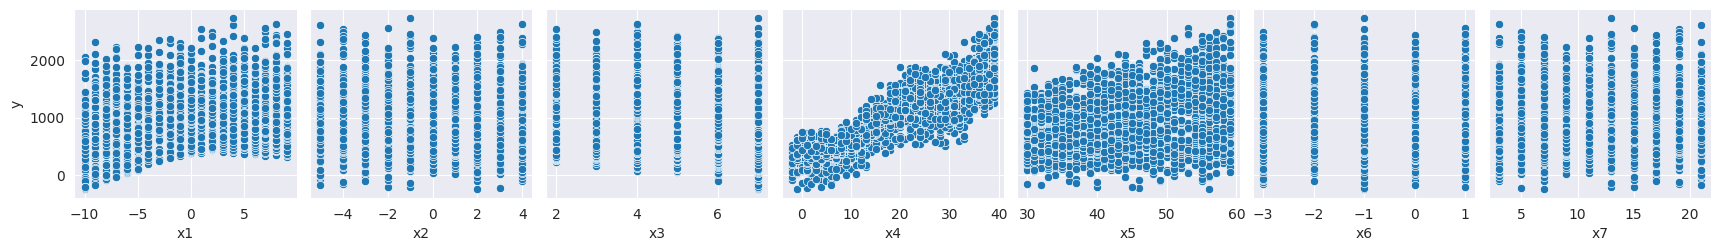
\includegraphics[width=\textwidth]{scatter.png}
    \caption{Wykresy punktowe 7 cech vs zmienna objaśniana}
\end{figure}
Pojawiła się następująca obserwacja -- $x_1, x_4, x_5$ powinny być istotne. Możemy w łatwy sposób sprawdzić tę hipotezę. Policzmy korelację tych zmiennych względem $y$.
Biblioteka \texttt{pandas} udostępnia nam funkcję \texttt{corr()}, która pod spodem korzysta z korelacji Pearsona.
\begin{figure}[h!]
    \centering
    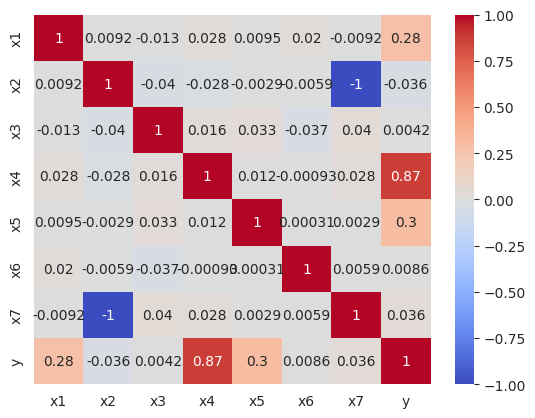
\includegraphics[width=0.55\textwidth]{corr.png}
    \caption{Macierz korelacji Pearsona}
\end{figure}
Rzeczywiście $x_1, x_4, x_5$ są istotne.

\section{Podział danych}
Dane podzieliłem w sposób losowy na 3 zbiory -- treningowy 60\%, walidacyjny 20\% oraz testowy 20\% z pomocą funkcji \texttt{numpy.shuffle()}. Takich podziałów wykonałem 10, żeby uśrednić wyniki -- coś na kształt walidacji krzyżowej.

\section{Pierwsze modele}
Celowo jeszcze nie skaluję danych. \\
Z wykładu wiemy, że dla prostej regresji możemy wyznaczyć $\theta$ analitycznie
\[ \theta = (X^T X)^{-1}X^T y,\]
gdzie $X$ i $y$ to odpowiednio macierz planowania i wektor zmiennej objaśnianej.
W przypadku bez $\theta_0$ nie dodajemy kolumny samych 1 do $X$. Jeśli $(X^T X)^{-1}$ nie istnieje to używamy pseudo-odwrotności Moore'a-Penrose'a -- \texttt{numpy.pinv()}. \\
Poprawność została sprawdzona przy użyciu biblioteki \texttt{SciKit-Learn}.

\subsection{Rozwiązanie analityczne bez $\theta_0$}
\begin{flalign*}
&\theta = [23.6648, -101.5721, -6.4955, 39.0517, 18.7345, -0.8390,-49.5116]^T &&\\
&\texttt{Training loss: } 14120.0796 &&\\
&\texttt{Validation loss: }  15464.2807 &&\\
&\texttt{Test loss: } 14883.7154
\end{flalign*}
\subsection{Rozwiązanie analityczne z $\theta_0$}
\begin{flalign*}
&\theta = [-22.0573, 23.6648, -97.5617, -6.4955, 39.0517, 18.7345, -0.8390, -47.5064]^T &&\\
&\texttt{Training loss: } 14120.0796 &&\\
&\texttt{Validation loss: } 15464.2807 &&\\
&\texttt{Test loss: } 14883.7154
\end{flalign*}
\subsection{Obserwacje}
Niezależnie od $\theta_0$ dostajemy te same błędy, te same $\theta_1, \theta_4, \theta_5$. \texttt{SciKit} to potwierdza. Mam podejrzenia, że jest to związane z tym, że $x_1, x_4, x_5$ na wykresach przechodzą przez początek układu współrzędnych, a inne zmienne nie mają większego znaczenia.

\section{Metoda spadku wzdłuż gradientu}
Od teraz rozpatruję modele tylko z $\theta_0$.
\subsection{Gradient Descent}
\[\theta^{[k+1]} \leftarrow \theta^{[k]} - \alpha \sum_{i=1}^{m}{(h_{\theta}(x^{(i)}) - y^{(i)})x^{(i)}}\]
Ustaliłem z góry liczbę iteracji na \texttt{EPOCHS = 3000}. \\
I tutaj był mój pierwszy błąd. Nie potrafiłem ustawić odpowiednio małego $\alpha$, gradient eksplodował. \\
Ostatecznie skończyłem z takim wzorem
\[\theta^{[k+1]} \leftarrow \theta^{[k]} - \frac{\alpha}{m}\sum_{i=1}^{m}{(h_{\theta}(x^{(i)}) - y^{(i)})x^{(i)}}.\]
Jak się później okazało, wystarczyło $\alpha \leftarrow \frac{\alpha}{m}$, żeby sama suma działała poprawnie. \\
Przy pomocy zbioru walidacyjnego, wyszło mi, że $\alpha = 0.0007$. \\
Spójrzmy jak to zbiega do minimum.
\begin{figure}[h!]
    \centering
    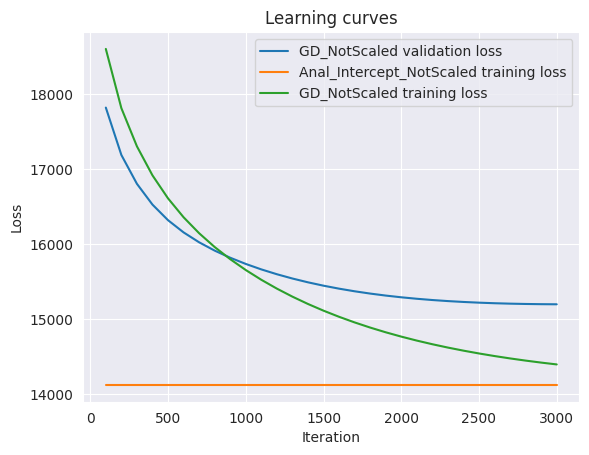
\includegraphics[width=0.5\textwidth]{gd_notscaled.png}
    \caption{Zbieżność GD}
\end{figure}
Jak widać na załączonym obrazku, zbiega powoli. Podejrzenia -- cechy nie są przeskalowane i gradient nie ma jednolitych spadków. \\
\textbf{Drobna uwaga:} tym razem poprawność sprawdziłem korzystając z definicji pochodnej
\[\nabla \mathcal{J}(\theta) =  \frac{\mathcal{J}(\theta + \epsilon) - \mathcal{J}(\theta - \epsilon)}{2\epsilon}.\]

\subsection{Standaryzacja cech}
Zastosowałem znany i lubiany wzór
\[x^{(i)} \leftarrow \frac{x^{(i)} - \overline{x}}{\sigma(x)},\]
wszystko w obrębie kolumny. Średnia i odchylenie standardowe liczone są tylko na podstawie zbioru treningowego. $y$-ki nie zostały poddane standaryzacji. \\
Dla $\alpha = 0.1$ błąd na zbiorze walidacyjnym jest najmniejszy. Zobaczmy jak teraz GD zbiega.
\begin{figure}[h!]
    \centering
    \begin{subfigure}[b]{0.45\textwidth}
        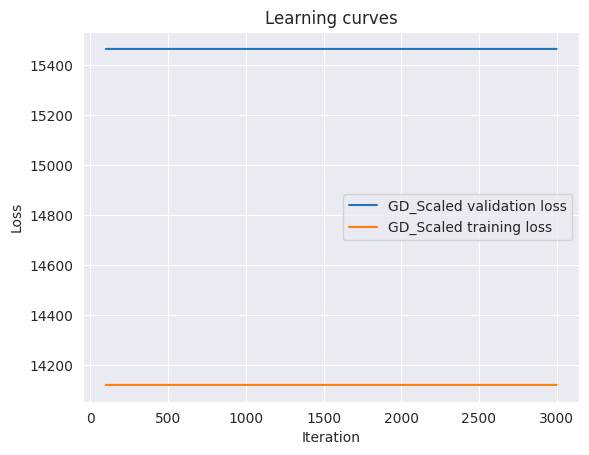
\includegraphics[width=\textwidth]{gd_scaled_parallel.png}
        \caption{\texttt{EPOCHS=3000}}
    \end{subfigure}
    \hfill
    \begin{subfigure}[b]{0.45\textwidth}
        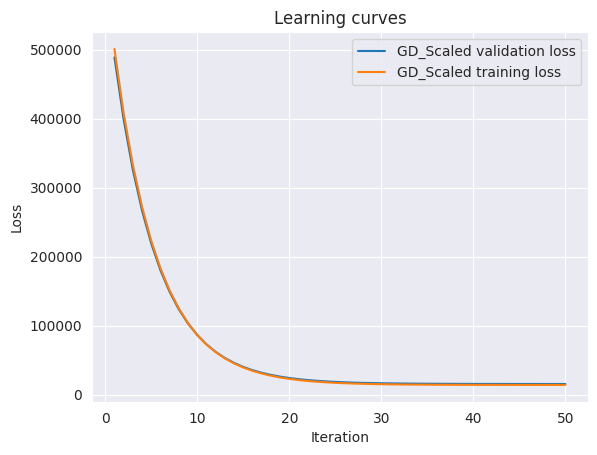
\includegraphics[width=\textwidth]{gd_scaled.png}
        \caption{\texttt{EPOCHS=50}}
    \end{subfigure}
\end{figure}
Standaryzowanie cech znacząco przyspiesza zbieżność, gradient wykonuje poprawny krok w wielu kierunkach.

\subsection{Stochastic Gradient Descent}
Od zwykłego GD różni się tylko tym, że zamiast całego zbioru treningowego losujemy jego podzbiór. Dokładając trochę probabila liczymy na to, że to się będzie lepiej uogólniać. \\
Empirycznie wyznaczyłem $\alpha=0.01$ oraz $\texttt{batch\_size}=64$. Zaciekawiła mnie mniejsza $\alpha$. Tłumaczę to sobie tym, że wylosowały się podzbiory z dużym krokiem gradientu i musieliśmy to zrównoważyć.
\begin{figure}[h!]
    \centering
    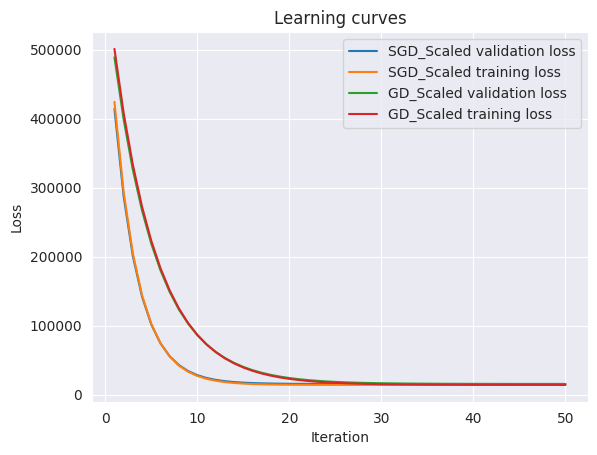
\includegraphics[width=0.55\textwidth]{gdvssgd.png}
    \caption{GD vs SGD}
\end{figure}
Jak widać SGD zbiega szybciej. Obie metody gradientowe dają podobne wyniki na zbiorze testowym.
\begin{flalign*}
&\texttt{Test loss [GD\_Scaled]: } 14853.6827 &&\\
&\texttt{Test loss [SGD\_Scaled]: } 14886.0377 &&
\end{flalign*}

\section{Regularyzacje}
Chcemy uniknąć zbytniego dopasowania do danych treningowych.
\subsection{Grzbietowa (L2)}
\[ \mathcal{J}(\theta) = \frac{1}{2} \sum_{i=1}^{m}{(h_{\theta}(x^{(i)}) - y^{(i)})^2 + \lambda \sum_{j=1}^{k}{\theta_j^2}} \]
Jak tak teraz patrzę na ten wzór to jest on inny niż na wykładzie i ja go świadomie zmieniłem, ponieważ analityczny nie brał średniej. Prawdopodobnie nie ma to znaczenia, wszystko nadrobią $\alpha, \lambda$.
\subsubsection{Rozwiązanie analityczne z $\theta_0$}
\begin{align*}
    &J = I \\
    &J[0,0] = 0 \\
    &\theta = (X^T X + \lambda J )^{-1}X^T y
\end{align*}
Stratę na jakimś zbiorze liczę już bez $||\theta_{-0}||_2^2$.
Taki model daje nam najlepszy wynik dla $\lambda = 1$ (trochę skłamałem, ponieważ sprawdziłem tylko do $\lambda=1$, a potem okazało się, że dla większych $\lambda$ jeszcze lepiej się uogólnia).

\subsubsection{SGD}
Hiperparametry: $\alpha=0.001, \texttt{babtch\_size}=64, \lambda=1$
\begin{figure}[h!]
    \centering
    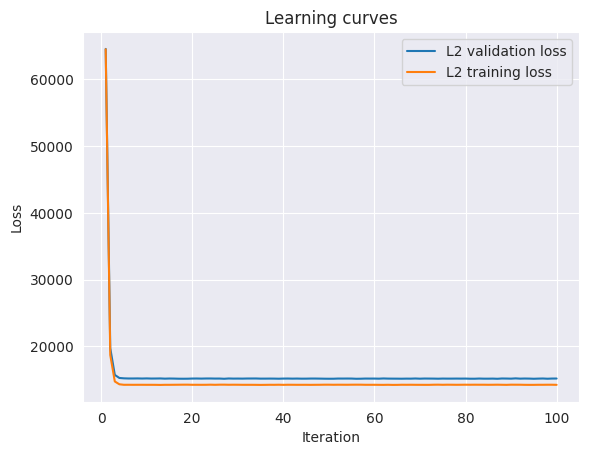
\includegraphics[width=0.55\textwidth]{l2sgd.png}
    \caption{L2 SGD}
\end{figure}
\\ Nieziemsko szybko zbiega do minimum.

\subsubsection{L2 SGD vs SGD}
Otrzymujemy mniejszą normę $\theta$ oraz mniejszy błąd na zbiorze testowym. Bardzo się cieszę, że tak wyszło.
\begin{flalign*}
&\texttt{Norm [Analytic\_Intercept\_Scaled]: } 507.8657 &&\\
&\texttt{Norm [L2]: } 492.7032 &&\\
&\texttt{Test loss [L2]: } 14496.2205 &&\\
&\texttt{Test loss [SGD\_Scaled]: } 14886.0377 &&\\
\end{flalign*}

\newpage

\subsection{Lasso (L1)}
\[ \mathcal{J}(\theta) = \sum_{i=1}^{m}{(h_{\theta}(x^{(i)}) - y^{(i)})^2 + \lambda \sum_{j=1}^{k}{|\theta_j|}} \]
Tutaj nie jesteśmy już w stanie użyć SGD.
\subsubsection{Spadek względem współrzędnych}
\begin{align*}
\hat{\theta}_j &= \argmin_{\theta_j \in \mathbb{R}} \sum_{i=1}^m \left( \theta^T x^{(i)} - y^{(i)} \right)^2 + \lambda \|\theta\|_1, \\
\\
\hat{\theta}_j &=
\begin{cases}
\frac{c_j + \lambda}{a_j} & \text{dla } c_j < -\lambda, \\
0 & \text{dla } c_j \in [-\lambda, \lambda], \\
\frac{c_j - \lambda}{a_j} & \text{dla } c_j > \lambda,
\end{cases} \\
\\
a_j &= 2 \sum_{i=1}^m \left(x_j^{(i)}\right)^2, \quad
c_j = 2 \sum_{i=1}^m \left( x_j^{(i)} y^{(i)} - \theta_{-j}^T x_{-j}^{(i)} \right)
\end{align*}
Ja pozwoliłem sobie ustawiać wszystkie $\theta_j$ w 1 iteracji.
\subsubsection{Wyniki}
Tutaj najbardziej oczekiwałem, że nieistotne cechy będą miały odpowiadające $\theta_i \approx 0$. \\
Hiperparametry: $\lambda = 256$
\begin{flalign*}
&\theta = [970.2551, 134.6390, -5.9474, -10.9890, 461.6880, 162.7735, -1.2059, 1.3487]^T &&
\end{flalign*}
Można powiedzieć, że efekt wyzerowania jest zadowalający.
\subsection{Sieć elastyczna (Elastic Net)}
\[ \mathcal{J}(\theta) = \sum_{i=1}^{m}{(h_{\theta}(x^{(i)}) - y^{(i)})^2} + \lambda\left( \alpha\sum_{j=1}^{k}{\theta_j^2} +
(1-\alpha)\sum_{j=1}^{k}{|\theta_j|} \right) \]
Korzystam z tego wzoru, ponieważ mogę rozszerzyć macierz planowania $X$ tak jak na ćwieczeniach i wrzucić do L1.

\subsection{SGD vs L2 vs L1 vs Elastic Net}
\begin{flalign*}
&\texttt{Test loss [ElasticNet]: } 14869.5227 &&\\
&\texttt{Test loss [L2]: } 14496.2205 &&\\
&\texttt{Test loss [L1]: } 14876.4765 &&\\
&\texttt{Test loss [SGD]: } 14886.0377 &&
\end{flalign*}
L2 króluje.
\section{Strata na zbiorze testowym względem rozmiaru zbioru treningowego}
\begin{figure}[h!]
    \centering
    \begin{subfigure}[b]{0.45\textwidth}
        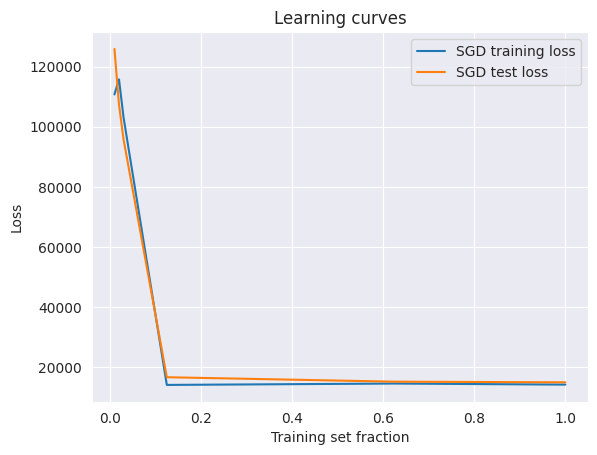
\includegraphics[width=\textwidth]{sgd_fast.png}
        \caption{$\alpha=0.01$}
    \end{subfigure}
    \hfill
    \begin{subfigure}[b]{0.45\textwidth}
        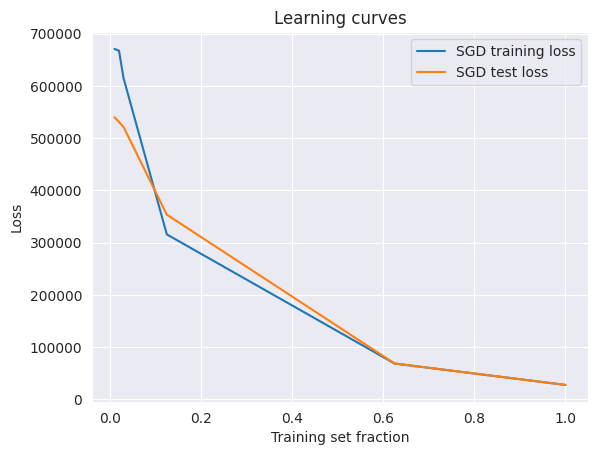
\includegraphics[width=\textwidth]{sgd_slow.png}
        \caption{$\alpha=0.1$}
    \end{subfigure}
    \caption{SGD}
\end{figure}
\begin{figure}[h!]
    \centering
    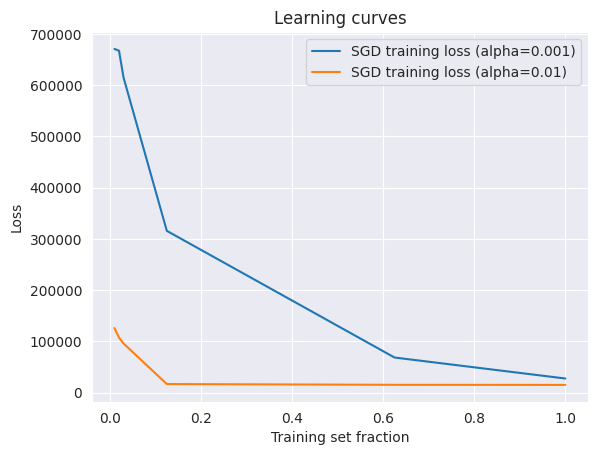
\includegraphics[width=0.4\textwidth]{sgd_converge_time.png}
    \caption{Zbieżność SGD}
\end{figure}

\newpage

\!\!\!\!\!\!\!\!\!Kolejny wykres wyjątkowo mi się podoba. \\
Pokazuje, że L2 najpierw się dopasowała a potem zaczęła regularyzację.
\begin{figure}[h!]
    \centering
    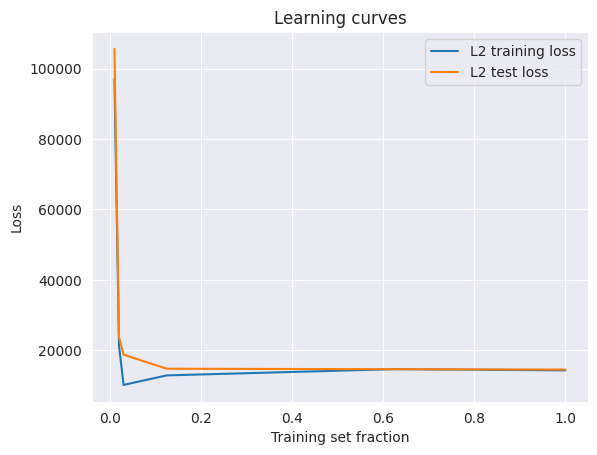
\includegraphics[width=0.4\textwidth]{l2_reg.png}
    \caption{Regularyzacja L2}
\end{figure}

\section{Dodatkowe funkcje bazowe}
Niestety w tej sekcji nie mogę się pochwalić wielkimi osiągnięciami. Zostawiłem $x_1, x_4, x_5$ w spokoju, a resztę zmiennych rozszerzyłem o wielomiany $x^2, x^3, x^4$ oraz $\sigma(x)$.
\begin{figure}[h!]
    \centering
    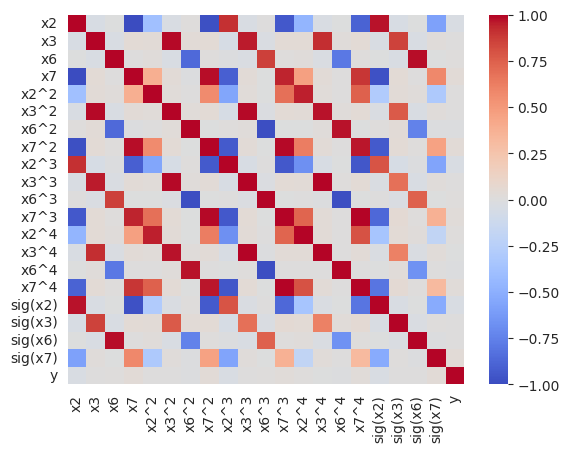
\includegraphics[width=0.8\textwidth]{aug_corr.png}
    \caption{Korelacja rozszerzonych zmiennych}
\end{figure}

\newpage

\!\!\!\!\!\!\!\!\!Macierz korelacji nie wróżyła nic ciekawego. \\
Puściłem na tym SGD z $\alpha=0.01$ i $\texttt{batch\_size}=64$. Ku mojemu zdziwieniu otrzymałem najlepszy wynik spośród wszystkich poprzednich.
\begin{flalign*}
&\texttt{Test loss [Augmented dataset SGD]: } 13369.6066 &&
\end{flalign*}

\section{Podsumowanie projektu}
Może nie otrzymałem satysfakcjonujących wyników na zbiorze testowym, ale zakochałem się bez pamięci w SGD i L2. To jest niesamowite jak dorzucenie odrobiny losowości poprawia wyniki. \\
\textbf{PS} \\
Proszę się nie gniewać za obrazek ze strony tytułowej, świetnie się bawiłem przy tym projekcie.

\section{BONUS}
\begin{figure}[h!]
    \centering
    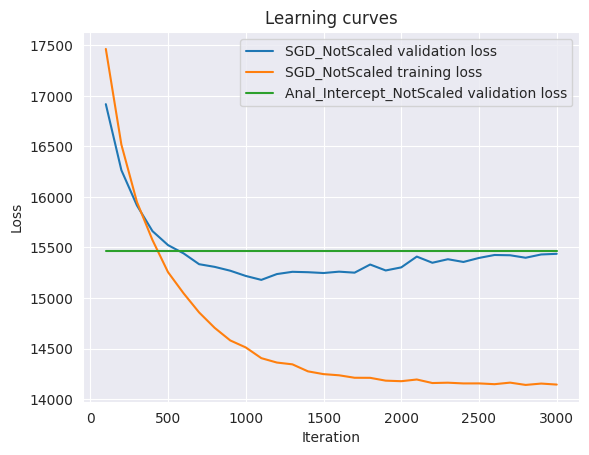
\includegraphics[width=0.8\textwidth]{bonus2.png}
    \caption{SGD schodzi poniżej analitycznej straty}
\end{figure}
\newpage
\begin{figure}[h!]
    \centering
    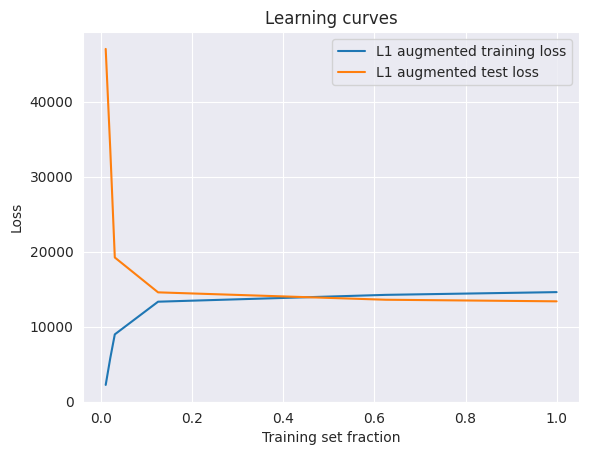
\includegraphics[width=0.8\textwidth]{bonus1.png}
    \caption{L1 z $\lambda=256$}
\end{figure}



% Bibliography (if required)
% \bibliographystyle{plain}
% \bibliography{references}  % Add a .bib file if you have references

\end{document}